\chapter{Introducción}


\section{El marketing digital en la web}


\subsection{¿Qué es el marketing digital?}

El marketing digital son técnicas y estrategias de comercialización usando medios digitales, tales como dispositivos móviles, televisiores digitales y ordenadores.

\vspace{5 mm}

\textbf{¿Cuáles son las principales diferencias respecto al marketing tradicional?}

\vspace{5 mm}

\begin{itemize}

\item \textbf{Personalización}: El marketing digital pretende obtener información del usuario más personalizada. Por ello, aplica técnicas que permiten que sugerir a los internautas información sobre aquello en lo que está interesado, basando estas recomendaciones en búsquedas previas o en sus preferencias definidas.

\item \textbf{Masivo}: Se puede obtener un gran número de usuarios que formen parte del público objetivo invirtiendo mucho menos dinero que en el marketing tradicional.


\end{itemize}

\subsection{Evolución}

El concepto de marketing digital ha ido ido variando desde sus inicios hasta la actualidad. En los años noventa, con la aparición de los primeros banners, aparecen las primeras técnicas de marketing en páginas web, aunque este primer concepto que se desarrolla es mucho más básico y se basaba principalmente en hacer publicidad hacia los usuarios para captar posibles clientes \cite{marketing-evolution}.

\vspace{5 mm}


Con la llegada de las redes sociales y la aparición de los smartphones, el concepto de marketing cambia: no se basa únicamente en promocionar un producto sino que se pretende crear una estrategia de venta basada en la perspectiva del cliente. Se reconoce e investiga en las áreas que ayuden a que los clientes piensen que sus opiniones importan, para  generar fidelidad hacia la marca. Aquí es donde las redes sociales juegan un gran papel, ya que permiten compartir todo tipo de contenido (videos, enlaces, textos) que se asocian a nuestras opiniones y gustos personales. Todo este contenido permite a las empresas conocer más detalladamente a un potencial cliente y así crear estrategías de marketing para fidelizarlo.


\subsection{Técnicas}

Disponer de una web es una de las mejores oportunidades para incrementar el prestigio y visibilidad de una marca y para alcanzar un mayor rango de clientes con efectividad. Para ello, entran en juego diversas técnicas de marketing digital que nos permiten obtener una mayor visibilidad de la marca o producto:

\vspace{5 mm}

\textbf{Posicionamiento SEO}

\vspace{5 mm}

\begin{figure}
\begin{center}
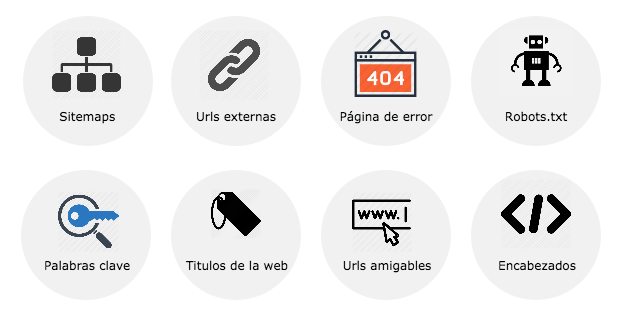
\includegraphics[width=1.0\textwidth]{imagenes/SEO.png}
\caption{Técnicas de SEO}
\label{SEO}
\end{center}
\end{figure}

El posicionamiento en buscadores mejor conocido como posicionamiento SEO es un conjunto de técnicas que implican una mejora de la página web con el fin de mejorar su posición en los resultados de los buscadores para unos términos de búsqueda específicos \cite{SEO}. Cuanto mejor esta optimizada la página web obtiene una mejor posición en los buscadores y por tanto una mayor visibilidad. En la figura \ref{SEO} se observan las principales técnicas de posicionamiento SEO, que se describen a continuación:

\begin{itemize}

\item \textbf{Uso de keywords}. Palabras clave, son un conjunto de datos asociados a la página que tienen relación con una posible búsqueda por parte de los usuarios en un buscador. Se asocian como metadatos a una página de la web y son unos de los elementos más básicos para el posicionamiento SEO.

\item \textbf{URL amigables}. Usar palabras cortas y amigables como Urls en el sitio web de vez de urls complejas, permite al buscador disponer de palabras clave para interpretar su contenido. Además es mucho más fácil de interpretar por las personas.

\item \textbf{Uso de etiquetas de título}. Cada página del sitio web, tiene unos metadatos asociados. Una de las etiquetas es el title(título), que indica el nombre de la página web. Es importante que cada página de la web tenga un título diferente y que el texto tenga una información relacionada con la página para facilitar la indexación por parte de los buscadores.

\item \textbf{Ofrecer un mapa de contenido del sitio a los robots buscadores}. Conocido como sitemaps(en inglés), es una lista de las páginas del sitio con información adicional tal como la importancia de la página o la frecuencia con la que cambia de contenidos. Generalmente los sitemaps se generan como fichero XML.

\item \textbf{Crear una página de error personalizada}. Una página de error amigable y personalizada mejora la experiencia para el usuario y evita problemas de indexación por parte de los buscadores.

\item \textbf{Insertar links externos}. Disponer de enlaces desde otras páginas consideradas por los buscadores también favorece  el buen posicionamiento de una web.

\item \textbf{Proporcionar un fichero robots.txt}. Fichero de texto que sirve de guía a los buscadores para rastrear  qué información del sitio hay que indexar a fin de posicionarla. Mediante este fichero se delimitan que páginas no queremos que aparezcan posicionadas (página de admin o de política de privacidad por ejemplo) y se facilita la lectura por parte de los crawlers(rastreadores) en el sitio.

\item \textbf{Ofrecer encabezados de la página}. Se deben utilizar las etiquetas de encabezado(h1,h2,h3) correctamente, estableciendo una jerarquía de la web y, de paso, que sean utilizadas como palabras clave.


\end{itemize}

\vspace{5 mm}

\textbf{La analítica web}

\vspace{5 mm}

La analítica web permite estudiar la repercusión de las campañas de marketing on-line. Con esta técnica se pretende entender el tráfico del sitio
web y así implementar nuevas mejoras.

\vspace{5 mm}

En los inicios de la analítica web, el objetivo principal consistía en medir el número de visitas a una determinada página. Cuantas más visitas,
existía una mayor probabilidad de generar impacto publicitario. En la actualidad se sigue analizando el número de visitas de un sitio, pero la analítica
web ha evolucionado y se miden otros indicadores, como la profundidad de las visitas. Las métricas más importantes utilizadas se dividen en dos tipos:
básicas y avanzadas.

\vspace{5 mm}

\textbf{Métricas básicas}: permiten ver el tráfico de usuarios de la web:

\begin{description}

\item \textbf{Sesiones}. Número de visitas que tiene la página.

\item \textbf{Visitas únicas}. Número de usuarios que han visto la página.

\item \textbf{Tasa de salida}. Conocer las páginas de la web en las que los visitantes abandonan la web.

\item \textbf{Usuarios}. Número de usuarios que visitan la web.

\item \textbf{Duración de la sesión}. Duración media de una sesión en la web.

\end{description}

\vspace{5 mm}

\textbf{Métricas avanzadas(KPI)}: indicadores clave del rendimiento del sitio web. Estás métricas se basan en la comparación de los objetivos marcados por la empresa con los resultados conseguidos. En función del tipo del sitio web, los objetivos serán diferentes y por tanto, los KPIs variaran. Algunos KPI son:

\begin{description}


\item [Tasa de conversión]. Porcentaje que se obtiene del número de conversiones que se producen a partir del número de visitas. La definición de conversión dependerá del tipo de web. Para un sitio con contenidos las conversiones son el número de registros en la aplicación. Para el caso de un e-commerce la tasa de conversión es la relación entre el número de ventas del sitio y el nº de visitantes.

\item [Fuentes de tráfico]. Analiza las fuentes de donde provienen las visitas de los usuarios. Las fuentes de tráfico pueden provenir de diferentes sitios:

\begin{itemize}
\item Búsqueda Orgánica(organic search): El usuario ha accedido a la web a través de buscadores como Google o Yahoo.
\item Búsqueda de pago(paid search): El usuario accede mediante enlaces directos de anuncios de herramientas de marketing como Adwords.
\item Tráfico directo: El usuario introduce la url directamente en el navegador.
\item Social: Proviene de redes sociales cómo Twitter,Facebook o Google+.
\item Referenciada: Los visitantes provienen de links directos de otras páginas.
\end{itemize}

\item [Tasa de rebote]. Porcentaje de visitas de una sola página. Es decir usuarios que visitan la página pero no interactúan con ella ya que la abandonan nada más visitarla.
\end{description}

\begin{figure}
\begin{center}
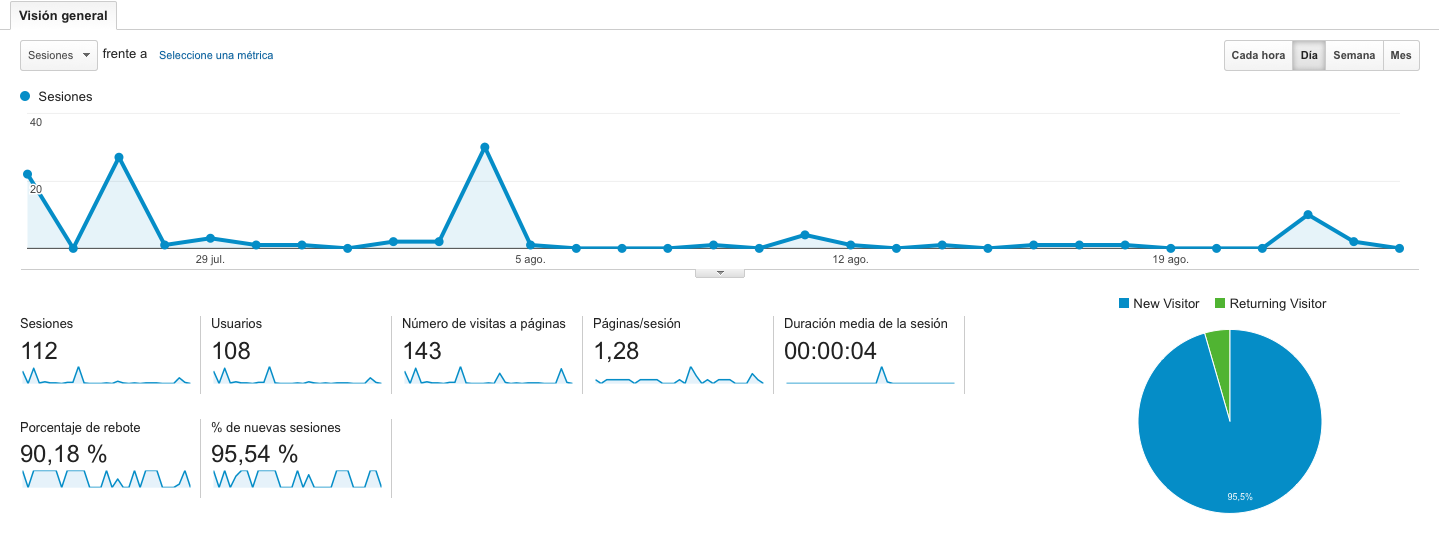
\includegraphics[width=1.0\textwidth]{imagenes/analytics.png}
\caption{Panel de Google Analytics}
\label{analytics}
\end{center}
\end{figure}

Para monitorizar toda el tráfico de datos obtenido de las métricas aplicadas se usan herramientas de analítica web. Una excelente herramienta gratuita es Google Analytics, que proporciona un dashboard o panel de control muy completo para monitorizar la información de un sitio web \cite{analytics}. Como se observa en la figura \ref{analytics} en Google Analytics se muestra toda la información de forma gráfica facilitando el análisis de los datos.

\vspace{5 mm}

\textbf{La redes sociales}

\vspace{5 mm}

Con la aparición de las redes sociales y su gran aceptación entre los usuarios de internet, las empresas han encontrado una herramienta muy potente para promover sus marcas. Las principales técnicas de social media marketing, adaptadas a las necesidades de cada empresa  pueden reportar muchos beneficios:

\begin{itemize}

\item \textbf{Difusión}: Se consigue una difusión de la información rápida y económica,

\item \textbf{Recopilación de datos}: se obtiene una gran cantidad de información(BIG DATA) sobre el público objetivo de la marca utilizando una táctica para las redes sociales.

\item \textbf{Mayor número de visitas}: mediante la difusión de contenido en redes sociales y con una buena táctica bien orientada, se consigue una mayor visibilidad del sitio web.

\end{itemize}

Como se ha expuesto anteriormente, del uso de tácticas de social media se obtiene una recopilación de datos relevante para ser utilizada por una empresa, con el fin de afianzar la fidelidad de sus clientes o de conseguir nuevos. Con los datos obtenidos de las redes sociales, las empresas pueden analizar la información y utilizarla adecuadamente para dar una mayor visibilidad a su marca. Un ejemplo de uso de los datos de redes sociales podría ser la obtención de un segmento del mercado, donde los potenciales clientes poseen unas características y necesidades similares(un nicho de mercado) sobre el que la empresa pueda generar un nuevo modelo de negocio \cite{social-media-marketing}.


\subsection{Targeting de las redes sociales}

Aunque todas las redes sociales se emplean generalmente para dar una mayor visibilidad, para conseguir un resultado satisfactorio, se debe elegir previamente la red social adecuada que usan los potenciales clientes del producto \cite{social-targetting}.

\vspace{5 mm}

Actualmente existen muchas redes sociales enfocadas a diferentes ámbitos: Linkedin(ámbito profesional), Pinterest(ámbito artistico) o Facebook(ámbito social). Cualquiera de las redes sociales actuales se puede emplear como ``target'' para llegar a un segmento de clientes. Si el `target'' incialmente no esta definido o engloba un grupo de usuarios muy heterogéneo, es más aconsejable escoger una red social con  un mayor número de usuarios ya que crea la posibilidad de ir acotando los distintos ``targets'' existentes y elegir el que más convenga para definir un nicho de mercado. Tres de las redes sociales más usadas en el mundo son: la web de microblogging Twitter, la web social de amistades Facebook y la aplicación de fotografía Instagram.

\vspace{5 mm}

\textbf{Twitter} probablemente sea la red social más adecuada para empezar a acotar un target sobre el que generar una nueva oportunidad de negocio.
La principal ventaja de Twitter son las datos en tiempo real que pueden publicar los usuarios(Tweets). Mediante los Tweets, las personas expresan sus
gustos,emociones, noticias relevantes, etc. Entre los temas o palabras más repetidos por los usuarios en el momento en una región determinada se generán
unas tendencias(Hashtags) que son una representación de los intereses comunes de unos usuarios para una región concreta. Cada una de las tendencias puede
ser un potencial target sobre el que la empresa puede crear una relacion fuerte con el usuario. Esta es la principal ventaja de Twitter respecto a las otras redes
sociales: la diversidad de temas en tiempo real.

\section{Big Data}

Una herramienta que está comenzando a utilizarse para obtener información sobre los usuarios y los mercados para así, generar mejores estrategias de marketing es el Big Data. Con esta técnica, los encargados de marketing de las
distintas empresas pueden conocer mejor sus clientes objetivo y mejorar tanto los productos que ofrecen como los mensajes que desean transmitirles.

\subsection{¿Qué es el Big Data?}

``Big Data'' se concibe como la gestión y análisis de grandes cantidades de información. El ``Big Data'' nos proporciona soluciones que utilizando métodos convencionales llevaría un tiempo mucho más elevado.

\subsection{Las tres uves del `BIG DATA''}

Todo el volumen de información puede provenir de diferentes tipos de fuentes. En Big data se definen 3 tipos de propiedades de los datos(ver figura \ref{3vs}):

\begin{itemize}

\item \textbf{Volumen de datos}: hace referencia a el tamaño de los datos.

\item \textbf{Variedad de datos}: se refiere a los distintos tipos de datos

\item \textbf{Velocidad de datos}: la velocidad con la que se procesan los datos.

\end{itemize}

\begin{figure}
\begin{center}
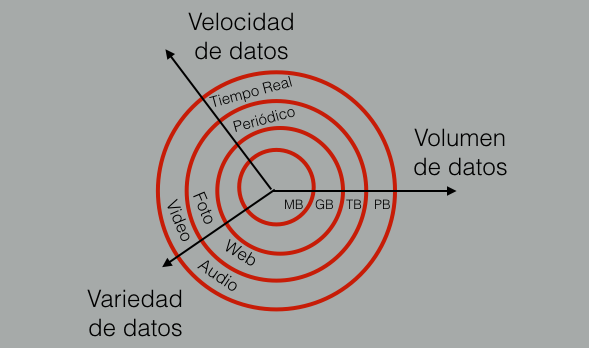
\includegraphics[width=1.0\textwidth]{imagenes/3V.png}
\caption{Las tres uves del Big Data}
\label{3vs}
\end{center}
\end{figure}

\subsection{Ventajas Principales}


\begin{itemize}
  \item \textbf{Reducción de costes}: Las tecnologías de ``Big Data'' pueden proporcionar una mayor rápidez a la hora de desarrollar el producto y permitir compartir datos de una manera más ágil.

  \item \textbf{Toma de decisiones rápida}: Manejando de forma apropiada la información que proporciona ``Big Data'' se podrán tomar
  decisiones más rápidas y eficientes.

  \item \textbf{Nuevos productos y servicios}: Con el análisis de ``Big Data'' se pueden desarrollar productos que cubran necesidades de los usuarios.

\end{itemize}

\subsection{Usos aplicables en las aplicaciones web}

Las principales fuentes de datos en la web son los usuarios. Estos proporcionan una información acerca de sus gustos y preferencias que son
recogidos y almacenados para posteriormente ser analizados por analistas de datos. Estos datos pueden ser usados en diversos ámbitos: \textbf{Empresarial}, \textbf{Deporte} o \textbf{Investigación}. En la web el campo más recurrente suele ser el Empresarial.

\vspace{5 mm}

Las empresas recogen los datos de sus propias webs y de las redes sociales. Utilizando técnicas como la mineria de datos, se obtienen patrones de comportamiento de los usuarios que son usados por las compañías para conseguir mayores beneficios económicos. Un ejemplo sería una web de comercio electrónico(e-commerce) que utilizaría la información de los usuarios para crear anuncios más personalizados incluyendo productos en el que el usuario ya está interesado, aumentando las probabilidades de compra por parte del cliente.


\section{Planteamiento del proyecto}

Actualmente existen millones de aplicaciones web donde existen varios objetivos: desde webs puramente informativas como landings o webs
corporativas donde el objetivo principal es dar a conocer algo, hasta un ecommerce donde el principal propósito es la venta de un producto. Para conseguir
que se cumplan los objetivos satisfactoriamente, son necesarios algunos factores internos como son la usabilidad o la fluidez de la aplicación. Pero existe
un factor externo que es muy imporante para que el proyecto web tenga éxito: la visibilidad, que no es más que conseguir destacar el contenido de
el sitio. La principal forma de destacar, es que la web aparezca en los principales buscadores web.

\vspace{5 mm}

Los buscadores se basan en las técnicas indexación de contenidos para mostrar el listado de páginas web ordenadas según la búsqueda del usuario.
Estas se basan en la recogida de datos semánticos de la web(crawling). Pero, ¿Es posible generar visibilidad mediante otra vía que no sean los buscadores
y segmentado por áreas?.

\vspace{5 mm}

Bajo este contexto surge la idea de NjoyCooking. Esta se concibe como una herramienta de marketing que pretende profundizar en el campo de la visibilidad web enfocado a webs de gastronomía y acotandolas sobre las distintas zonas o áreas geográficas.
